% =====================================================================
% Clase -- Geometría 6° -- Trimestre I -- Semana 04
% Sesión 003 (lun 21 sep., 13:40, 50 min)
% Tema: Ángulos
% Subtema: Estimar ángulos con referentes; el ángulo de tiro
% Hilo conductor del trimestre I: «La geometría del fútbol»
% Tema 1 de la guía: Ángulos (tema:angulos)
% Material del docente (no se entrega a los estudiantes).
% =====================================================================
\documentclass[11pt]{article}
\makeatletter\def\input@path{{../../../../../plantillas/estilo/}}\makeatother
\usepackage{mmcantillo}
\guiadelestudiante{../../guia-didactica/guia-periodo-I-angulos-poligonos}

\tipodocumento{Clase}
\asignatura{Geometría}
\titulo{Semana 4: ¿desde dónde es más fácil hacer gol?}
\grado{6°}
\periodo{I}

% DBA: matematicas grado 6 · DBA 5 — Propone y desarrolla estrategias de estimación, medición
% y cálculo de diferentes cantidades (ángulos, longitudes, áreas, volúmenes, etc.) para
% resolver problemas. Evidencias de esta sesión: «Estima el resultado de una medición sin
% realizarla, de acuerdo con un referente previo» y «Decide acerca de las estrategias para
% determinar qué tan pertinente es la estimación y analiza las causas de error».

\begin{document}

\encabezado*

\begin{center}
{\renewcommand{\arraystretch}{1.3}
\begin{tabularx}{\linewidth}{@{}l l l X l@{}}
  \toprule
  \textbf{Sesión} & \textbf{Fecha} & \textbf{Min} & \textbf{Subtema} & \textbf{Entregables}\\
  \midrule
  003 & lun 21 sep., 13:40 & 50 & Estimar ángulos con referentes; el ángulo de tiro
      & Taller (5 puntos)\\
  \bottomrule
\end{tabularx}}
\end{center}

Cierre del tema 1. En las dos sesiones anteriores se clasificaron y se midieron ángulos; hoy
se aprende a \emph{estimarlos} antes de medir —usando el ángulo recto como vara de medir— y se
resuelve la discusión del portero y el delantero con la que abrió el trimestre.
Referencia: \refguia{tema:angulos}.

% ---------------------------------------------------------------------
\seccion{Sesión 003 — lunes 21 de septiembre · 13:40 · 50 min}

\textbf{Objetivo.} Estimar la medida de un ángulo usando referentes, comprobar la estimación
con el transportador y juzgar si el error es aceptable; aplicarlo al ángulo de tiro.

\textbf{Materiales.} Tablero; transportador, regla y escuadra; una hoja cuadriculada por
estudiante; la guía. Si hay cancha o patio a la vista, mejor.

\begin{center}
{\renewcommand{\arraystretch}{1.3}
\begin{tabularx}{\linewidth}{@{}l l X@{}}
  \toprule
  \textbf{Momento} & \textbf{Min} & \textbf{Actividad}\\
  \midrule
  Enganche & 0--6 & Volver a la pregunta del trimestre: el portero dice que desde el punto
    penal «es imposible fallar» y el delantero que desde la esquina «tampoco es tan
    difícil». ¿Quién tiene razón? Anotar en el tablero las apuestas del curso.\\
  Estimar & 6--18 & El ángulo recto como referente: la esquina del cuaderno, la escuadra.
    Dibujar cinco ángulos en el tablero y pedir la estimación a mano alzada («¿más o menos
    que un recto? ¿la mitad? ¿el doble?»). Solo después medir uno con el transportador y
    calcular el error. Regla de la clase: \textbf{una estimación sirve si se aleja menos
    de $10^\circ$}.\\
  Medir & 18--28 & Repaso rápido del transportador (centro en el vértice, cero sobre un
    lado, cuál de las dos escalas leer). Errores típicos: leer la escala equivocada y no
    apoyar el centro. Cada uno mide dos de los ángulos del tablero.\\
  Taller & 28--47 & Taller individual (5 puntos). Las preguntas 3 y 4 piden dibujar a
    escala: $\qty{1}{cm}$ por metro en la hoja cuadriculada. Quien no traiga transportador
    trabaja en pareja.\\
  Cierre & 47--50 & Recoger el taller. Resolver la apuesta del inicio con los números que
    salieron. Anuncio: la próxima clase, las líneas de la cancha (rectas paralelas y
    perpendiculares).\\
  \bottomrule
\end{tabularx}}
\end{center}

\textbf{Figura para el tablero: el ángulo de tiro.}

\begin{center}
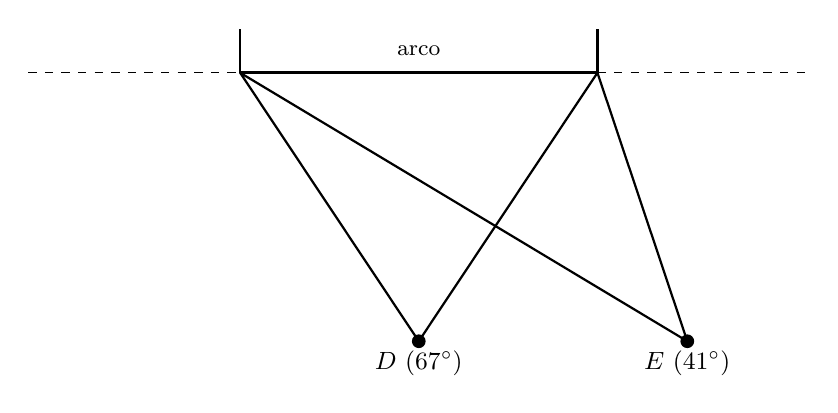
\begin{tikzpicture}[scale=0.62, every node/.style={font=\small}]
  % arco: postes en (-3.66, 0) y (3.66, 0)
  \draw[very thick] (-3.66,0) -- (3.66,0);
  \draw[thick] (-3.66,0) -- (-3.66,0.9);
  \draw[thick] (3.66,0) -- (3.66,0.9);
  \draw[dashed] (-8,0) -- (-3.66,0); \draw[dashed] (3.66,0) -- (8,0);
  \node at (0,0.45) {\footnotesize arco};
  % jugador D, de frente a 5,5 m
  \coordinate (D) at (0,-5.5);
  \draw[thick] (D) -- (-3.66,0); \draw[thick] (D) -- (3.66,0);
  \fill (D) circle (4pt) node[below] {$D$ (67$^\circ$)};
  % jugador E, corrido 5,5 m
  \coordinate (E) at (5.5,-5.5);
  \draw[thick] (E) -- (-3.66,0); \draw[thick] (E) -- (3.66,0);
  \fill (E) circle (4pt) node[below] {$E$ (41$^\circ$)};
\end{tikzpicture}

{\small Los dos están a $\qty{5,5}{m}$ de la línea de meta. No es lo mismo la distancia que
la posición.}
\end{center}

\begin{nota}
\textbf{El punto de la clase.} Casi todo el curso va a apostar por «el que esté más cerca».
La figura muestra que dos jugadores a la \emph{misma} distancia pueden tener ángulos muy
distintos: $67^\circ$ de frente contra $41^\circ$ corrido hacia un lado. Vale la pena dejar
la pregunta abierta —«¿y si se aleja pero se centra?»— porque el punto de mejor ángulo no
está pegado al arco; se retoma en 7° con los teselados y las rotaciones.
\end{nota}

\begin{nota}
\textbf{Sobre el error.} La regla de los $10^\circ$ es un acuerdo de clase, no una verdad
matemática: sirve para que la palabra «error» tenga un significado concreto y medible. Si el
grupo estima muy bien, súbele la exigencia a $5^\circ$ en la próxima sesión.
\end{nota}

\end{document}
